\documentclass{standalone}
\usepackage{tikz}
\usetikzlibrary{patterns, positioning}


\begin{document}
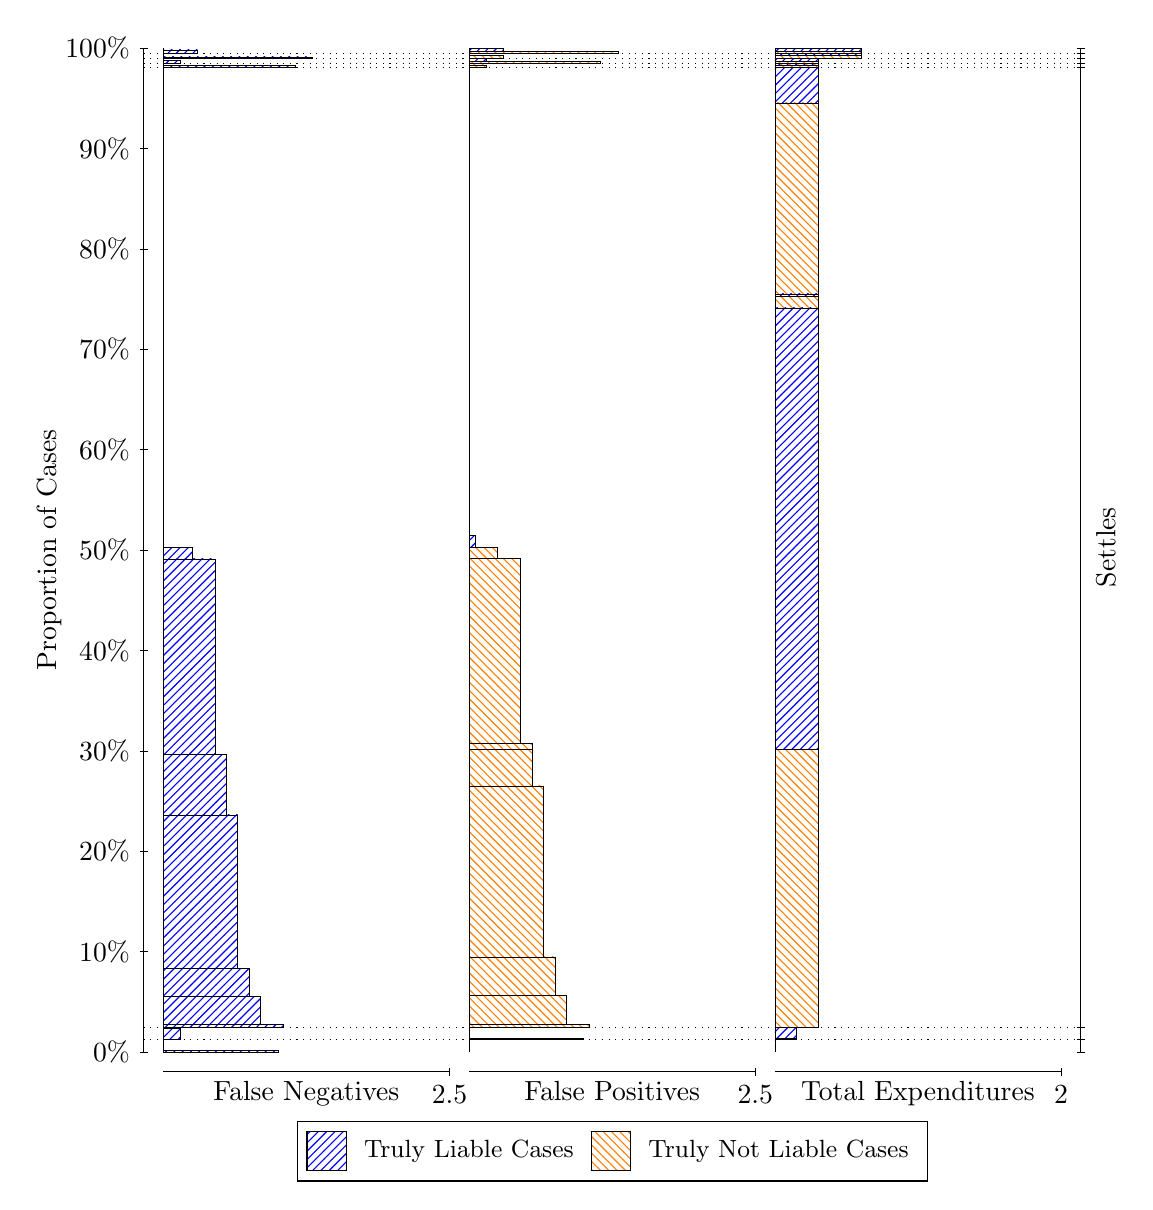
\begin{tikzpicture}
\draw[black, very thin] (1.5,1.75) -- (1.5,14.5);
\node[rotate=90, text=black, anchor=center] at (0.3, 8.125) {Proportion of Cases};
\draw[black, very thin] (1.45,1.75) -- (1.55,1.75);
\node[text=black, anchor=east] at (1.45, 1.75) {0\%};
\draw[black, very thin] (1.45,3.025) -- (1.55,3.025);
\node[text=black, anchor=east] at (1.45, 3.025) {10\%};
\draw[black, very thin] (1.45,4.3) -- (1.55,4.3);
\node[text=black, anchor=east] at (1.45, 4.3) {20\%};
\draw[black, very thin] (1.45,5.575) -- (1.55,5.575);
\node[text=black, anchor=east] at (1.45, 5.575) {30\%};
\draw[black, very thin] (1.45,6.85) -- (1.55,6.85);
\node[text=black, anchor=east] at (1.45, 6.85) {40\%};
\draw[black, very thin] (1.45,8.125) -- (1.55,8.125);
\node[text=black, anchor=east] at (1.45, 8.125) {50\%};
\draw[black, very thin] (1.45,9.4) -- (1.55,9.4);
\node[text=black, anchor=east] at (1.45, 9.4) {60\%};
\draw[black, very thin] (1.45,10.675) -- (1.55,10.675);
\node[text=black, anchor=east] at (1.45, 10.675) {70\%};
\draw[black, very thin] (1.45,11.95) -- (1.55,11.95);
\node[text=black, anchor=east] at (1.45, 11.95) {80\%};
\draw[black, very thin] (1.45,13.225) -- (1.55,13.225);
\node[text=black, anchor=east] at (1.45, 13.225) {90\%};
\draw[black, very thin] (1.45,14.5) -- (1.55,14.5);
\node[text=black, anchor=east] at (1.45, 14.5) {100\%};

\draw[black, very thin] (13.4,1.75) -- (13.4,14.5);
\draw[black, very thin] (13.35,1.75) -- (13.45,1.75);
\node[anchor=west] at (13.35, 1.75) {};
\draw[black, very thin] (13.35,1.9082) -- (13.45,1.9082);
\node[anchor=west] at (13.35, 1.9082) {};
\draw[black, very thin] (13.35,2.0663) -- (13.45,2.0663);
\node[anchor=west] at (13.35, 2.0663) {};
\draw[black, very thin] (13.35,14.257) -- (13.45,14.257);
\node[anchor=west] at (13.35, 14.257) {};
\draw[black, very thin] (13.35,14.308) -- (13.45,14.308);
\node[anchor=west] at (13.35, 14.308) {};
\draw[black, very thin] (13.35,14.365) -- (13.45,14.365);
\node[anchor=west] at (13.35, 14.365) {};
\draw[black, very thin] (13.35,14.433) -- (13.45,14.433);
\node[anchor=west] at (13.35, 14.433) {};
\draw[black, very thin] (13.35,14.5) -- (13.45,14.5);
\node[anchor=west] at (13.35, 14.5) {};

\draw[black, very thin, pattern color=blue, pattern=north east lines] (1.75,1.75) rectangle (3.2033,1.7666);
\draw[black, very thin, pattern color=orange, pattern=north west lines] (1.75,1.7666) rectangle (1.75,1.9082);
\draw[black, very thin, pattern color=blue, pattern=north east lines] (1.75,1.9082) rectangle (1.968,2.0497);
\draw[black, very thin, pattern color=orange, pattern=north west lines] (1.75,2.0497) rectangle (1.75,2.0663);
\draw[black, very thin, pattern color=blue, pattern=north east lines] (1.75,2.0663) rectangle (3.276,2.0987);
\draw[black, very thin, pattern color=blue, pattern=north east lines] (1.75,2.0987) rectangle (2.9853,2.4556);
\draw[black, very thin, pattern color=blue, pattern=north east lines] (1.75,2.4556) rectangle (2.84,2.8121);
\draw[black, very thin, pattern color=blue, pattern=north east lines] (1.75,2.8121) rectangle (2.6947,4.7612);
\draw[black, very thin, pattern color=blue, pattern=north east lines] (1.75,4.7612) rectangle (2.5493,5.529);
\draw[black, very thin, pattern color=blue, pattern=north east lines] (1.75,5.529) rectangle (2.404,8.0127);
\draw[black, very thin, pattern color=blue, pattern=north east lines] (1.75,8.0127) rectangle (2.1133,8.1602);
\draw[black, very thin, pattern color=orange, pattern=north west lines] (1.75,8.1602) rectangle (1.75,14.257);
\draw[black, very thin, pattern color=blue, pattern=north east lines] (1.75,14.257) rectangle (3.4213,14.278);
\draw[black, very thin, pattern color=orange, pattern=north west lines] (1.75,14.278) rectangle (1.75,14.308);
\draw[black, very thin, pattern color=blue, pattern=north east lines] (1.75,14.308) rectangle (1.968,14.342);
\draw[black, very thin, pattern color=orange, pattern=north west lines] (1.75,14.342) rectangle (1.75,14.365);
\draw[black, very thin, pattern color=blue, pattern=north east lines] (1.75,14.365) rectangle (3.6393,14.388);
\draw[black, very thin, pattern color=orange, pattern=north west lines] (1.75,14.388) rectangle (1.75,14.433);
\draw[black, very thin, pattern color=blue, pattern=north east lines] (1.75,14.433) rectangle (2.186,14.477);
\draw[black, very thin, pattern color=orange, pattern=north west lines] (1.75,14.477) rectangle (1.75,14.5);
\draw[black, very thin, pattern color=orange, pattern=north west lines] (5.6333,1.75) rectangle (5.6333,1.8915);
\draw[black, very thin, pattern color=blue, pattern=north east lines] (5.6333,1.8915) rectangle (5.6333,1.9082);
\draw[black, very thin, pattern color=orange, pattern=north west lines] (5.6333,1.9082) rectangle (7.0867,1.9248);
\draw[black, very thin, pattern color=blue, pattern=north east lines] (5.6333,1.9248) rectangle (5.6333,2.0663);
\draw[black, very thin, pattern color=orange, pattern=north west lines] (5.6333,2.0663) rectangle (7.1593,2.0987);
\draw[black, very thin, pattern color=orange, pattern=north west lines] (5.6333,2.0987) rectangle (6.8687,2.4697);
\draw[black, very thin, pattern color=orange, pattern=north west lines] (5.6333,2.4697) rectangle (6.7233,2.9568);
\draw[black, very thin, pattern color=orange, pattern=north west lines] (5.6333,2.9568) rectangle (6.578,5.1303);
\draw[black, very thin, pattern color=orange, pattern=north west lines] (5.6333,5.1303) rectangle (6.4327,5.5904);
\draw[black, very thin, pattern color=orange, pattern=north west lines] (5.6333,5.5904) rectangle (6.4327,5.6681);
\draw[black, very thin, pattern color=orange, pattern=north west lines] (5.6333,5.6681) rectangle (6.2873,8.0152);
\draw[black, very thin, pattern color=orange, pattern=north west lines] (5.6333,8.0152) rectangle (5.9967,8.1627);
\draw[black, very thin, pattern color=blue, pattern=north east lines] (5.6333,8.1627) rectangle (5.706,8.3102);
\draw[black, very thin, pattern color=blue, pattern=north east lines] (5.6333,8.3102) rectangle (5.6333,14.257);
\draw[black, very thin, pattern color=orange, pattern=north west lines] (5.6333,14.257) rectangle (5.8513,14.287);
\draw[black, very thin, pattern color=blue, pattern=north east lines] (5.6333,14.287) rectangle (5.6333,14.308);
\draw[black, very thin, pattern color=orange, pattern=north west lines] (5.6333,14.308) rectangle (7.3047,14.331);
\draw[black, very thin, pattern color=blue, pattern=north east lines] (5.6333,14.331) rectangle (5.8513,14.365);
\draw[black, very thin, pattern color=orange, pattern=north west lines] (5.6333,14.365) rectangle (6.0693,14.409);
\draw[black, very thin, pattern color=blue, pattern=north east lines] (5.6333,14.409) rectangle (5.6333,14.433);
\draw[black, very thin, pattern color=orange, pattern=north west lines] (5.6333,14.433) rectangle (7.5227,14.456);
\draw[black, very thin, pattern color=blue, pattern=north east lines] (5.6333,14.456) rectangle (6.0693,14.5);
\draw[black, very thin, pattern color=orange, pattern=north west lines] (9.5167,1.75) rectangle (9.5167,1.8915);
\draw[black, very thin, pattern color=blue, pattern=north east lines] (9.5167,1.8915) rectangle (9.5167,1.9082);
\draw[black, very thin, pattern color=orange, pattern=north west lines] (9.5167,1.9082) rectangle (9.7892,1.9248);
\draw[black, very thin, pattern color=blue, pattern=north east lines] (9.5167,1.9248) rectangle (9.7892,2.0663);
\draw[black, very thin, pattern color=orange, pattern=north west lines] (9.5167,2.0663) rectangle (10.062,5.5904);
\draw[black, very thin, pattern color=blue, pattern=north east lines] (9.5167,5.5904) rectangle (10.062,11.199);
\draw[black, very thin, pattern color=orange, pattern=north west lines] (9.5167,11.199) rectangle (10.062,11.347);
\draw[black, very thin, pattern color=blue, pattern=north east lines] (9.5167,11.347) rectangle (10.062,11.379);
\draw[black, very thin, pattern color=orange, pattern=north west lines] (9.5167,11.379) rectangle (10.062,13.804);
\draw[black, very thin, pattern color=blue, pattern=north east lines] (9.5167,13.804) rectangle (10.062,14.257);
\draw[black, very thin, pattern color=orange, pattern=north west lines] (9.5167,14.257) rectangle (10.062,14.287);
\draw[black, very thin, pattern color=blue, pattern=north east lines] (9.5167,14.287) rectangle (10.062,14.308);
\draw[black, very thin, pattern color=orange, pattern=north west lines] (9.5167,14.308) rectangle (10.062,14.331);
\draw[black, very thin, pattern color=blue, pattern=north east lines] (9.5167,14.331) rectangle (10.062,14.365);
\draw[black, very thin, pattern color=orange, pattern=north west lines] (9.5167,14.365) rectangle (10.607,14.409);
\draw[black, very thin, pattern color=blue, pattern=north east lines] (9.5167,14.409) rectangle (10.607,14.433);
\draw[black, very thin, pattern color=orange, pattern=north west lines] (9.5167,14.433) rectangle (10.607,14.456);
\draw[black, very thin, pattern color=blue, pattern=north east lines] (9.5167,14.456) rectangle (10.607,14.5);
\draw[black, dotted] (1.5,1.9082) -- (13.4,1.9082);
\draw[black, dotted] (1.5,2.0663) -- (13.4,2.0663);
\draw[black, dotted] (1.5,14.257) -- (13.4,14.257);
\draw[black, dotted] (1.5,14.308) -- (13.4,14.308);
\draw[black, dotted] (1.5,14.365) -- (13.4,14.365);
\draw[black, dotted] (1.5,14.433) -- (13.4,14.433);
\draw[black, very thin] (1.75,1.5) -- (5.3833,1.5);
\node[text=black, anchor=north] at (3.5667, 1.5) {False Negatives};
\draw[black, very thin] (5.3833,1.45) -- (5.3833,1.55);
\node[text=black, anchor=north] at (5.3833, 1.45) {2.5};

\draw[black, very thin] (5.6333,1.5) -- (9.2667,1.5);
\node[text=black, anchor=north] at (7.45, 1.5) {False Positives};
\draw[black, very thin] (9.2667,1.45) -- (9.2667,1.55);
\node[text=black, anchor=north] at (9.2667, 1.45) {2.5};

\draw[black, very thin] (9.5167,1.5) -- (13.15,1.5);
\node[text=black, anchor=north] at (11.333, 1.5) {Total Expenditures};
\draw[black, very thin] (13.15,1.45) -- (13.15,1.55);
\node[text=black, anchor=north] at (13.15, 1.45) {2};



\node[text=black, centered, rotate=90] at (13.72, 8.1615) {Settles};





\draw (7.449999999999999,1.5) node[draw=none] (baseCoordinate) {};
\begin{scope}[align=center]
        \matrix[scale=0.5, draw=black, below=0.5cm of baseCoordinate, nodes={draw}, column sep=0.1cm]{
            \node[rectangle, draw, minimum width=0.5cm, minimum height=0.5cm, pattern color=blue, pattern=north east lines] {}; &
            \node[draw=none, font=\small, text=black] (B) {Truly Liable Cases}; &
            \node[rectangle, draw, minimum width=0.5cm, minimum height=0.5cm, pattern color=orange, pattern=north west lines] {}; &
            \node[draw=none, font=\small, text=black] (B) {Truly Not Liable Cases}; \\
            };
\end{scope}

\end{tikzpicture}
\end{document}